\documentclass{article}

\usepackage{microtype}
\usepackage{graphicx}
\usepackage{subfigure}
\usepackage{booktabs}
\usepackage{hyperref}
\usepackage[accepted]{icml2023}
\usepackage{amsmath}
\usepackage{amssymb}
\usepackage{xcolor}

\icmltitlerunning{YOLOv8 for Web UI Element Detection: A CNN Ablation Study}

\begin{document}

\twocolumn[
\icmltitle{YOLOv8 for Web UI Element Detection:\\A CNN Ablation Study}

\icmlsetsymbol{equal}{*}

\begin{icmlauthorlist}
\icmlauthor{Alden Bernstein}{ucsd}
\end{icmlauthorlist}

\icmlaffiliation{ucsd}{Department of Cognitive Science, University of California San Diego, La Jolla, CA, USA}

\icmlcorrespondingauthor{Alden Bernstein}{abernstein@ucsd.edu}

\icmlkeywords{convolutional neural networks, object detection, YOLO, UI element detection}

\vskip 0.3in
]

% skip \printAffiliationsAndNotice to remove fake ICML footer

% ============================================================
\begin{abstract}
We apply YOLOv8, a convolutional neural network (CNN) for object detection, to the task of localizing UI elements in web page screenshots. We crawl $\sim$260K screenshots from the Tranco Top~1M websites and conduct \textbf{14 controlled ablation experiments} covering (a)~architectures (YOLOv8n/s/m and a custom model), (b)~network depth, (c)~optimizers (SGD vs.\ AdamW), (d)~pooling (max vs.\ average), and (e)~activation functions (SiLU vs.\ ReLU), plus learning rate, resolution, augmentation, and initialization. We find that architecture choice dominates all other hyperparameters, but the biggest improvement comes from \textbf{data preparation}: consolidating 16 noisy classes into a single \texttt{ui\_element} class with deduplication and diverse sampling improves mAP50 from 0.136 (best 5-class) to \textbf{0.323} (1-class)---a 2.4$\times$ gain using the same model. This confirms OmniParser's~\cite{omniparser} single-class approach on independent data. We also train a text classifier for a practical application beyond the core CNN work. Development of the report and scripts was assisted by Claude Code.
\end{abstract}

% ============================================================
\section{Introduction}

For this project we wanted to apply CNN-based object detection to a non-standard dataset rather than a typical benchmark like CIFAR-10 or ImageNet. We chose web UI element detection---finding buttons, links, inputs, and other interactive elements in screenshots of websites---because (1)~we could crawl our own training data at scale, and (2)~OmniParser~\cite{omniparser} recently showed that YOLOv8 works well for this task, giving us a baseline to replicate and extend.

The practical motivation is browser agent security: LLM-powered agents~\cite{browseruse} that navigate websites can be tricked by hidden elements in the DOM~\cite{greshake2023}. A CNN that detects elements from the rendered screenshot only sees what is actually visible, naturally filtering hidden attacks. But for this report, our main focus is the CNN ablation study itself---systematically testing how different hyperparameter choices affect detection performance, as we did with simpler CNNs in the homework assignments.

We conduct 14 experiments varying one factor at a time, covering all five hyperparameter categories from the project guidelines: (a)~architectures, (b)~number of layers, (c)~optimizers, (d)~pooling functions, and (e)~activation functions. After finding that data quality mattered more than any hyperparameter, we iterated on the data pipeline (16 classes $\to$ 5 classes $\to$ 1 class with cleaning), achieving a 2.4$\times$ improvement over our best ablation result.

% ============================================================
\section{Related Work}

\textbf{CNN architectures} have been a focus throughout this course. ResNet~\cite{resnet} showed that skip connections enable training very deep networks. VGG~\cite{vgg} demonstrated that stacking small 3$\times$3 filters works better than larger kernels. MobileNet~\cite{mobilenet} introduced depthwise separable convolutions for efficient mobile inference. DenseNet~\cite{densenet} connected every layer to every other layer for feature reuse. These ideas---depth, filter design, efficiency, connectivity---all show up in YOLOv8's architecture.

\textbf{YOLOv8}~\cite{yolov8} is a single-stage object detector that predicts bounding boxes and class labels in one forward pass. It uses a CSPDarknet53 backbone with C2f blocks (a form of residual connection), a Feature Pyramid Network neck for multi-scale detection, and Spatial Pyramid Pooling (SPPF) for capturing context at multiple scales. We chose it because OmniParser~\cite{omniparser} showed it works for UI detection, and because it lets us ablate the same CNN components we studied in class (pooling, activation functions, depth, etc.).

\textbf{OmniParser}~\cite{omniparser, omniparserv2} fine-tunes a YOLO model on UI screenshots for screen parsing, using a single ``icon'' class. They combine this with OCR and captioning for a full pipeline. We replicate the single-class detection approach on our own independently crawled dataset and provide a systematic ablation that OmniParser did not include.

% ============================================================
\section{Method}

\subsection{Dataset}
\label{sec:dataset}

We built a Playwright-based web crawler that visits websites from the Tranco Top~1M ranking, takes screenshots at 1920$\times$1080 (top, mid, and bottom viewport sections), and extracts bounding box annotations from DOM element positions. This produced $\sim$260K annotated images. A separate pre-existing set of 668 annotated screenshots is used for validation and test splits, ensuring zero overlap with crawled training data.

\textbf{Class refinement (16 $\to$ 5 $\to$ 1).} The crawler initially produced 16 fine-grained classes (link, button, input, checkbox, etc.). We found severe class imbalance---the top~3 classes comprised 66\% of all annotations while the bottom~6 contributed $<$1\%. We first merged these into 5 groups for the ablation study, but per-class results showed that only 2 of 5 groups achieved meaningful detection (Table~\ref{tab:yolo_perclass}). Following OmniParser's approach~\cite{omniparser}, we then consolidated everything into a single \texttt{ui\_element} class, removed duplicate and tiny bounding boxes, and selected 1 image per domain for diversity ($\sim$47K training images). This iterative data cleaning turned out to be more impactful than any hyperparameter change.

\subsection{CNN Architecture: YOLOv8}
\label{sec:architecture}

YOLOv8 is a fully convolutional network with three parts, each containing components we ablate:

\textbf{Backbone (CSPDarknet53).} Convolutional layers with Cross-Stage Partial connections extract features at multiple scales through stride-2 downsampling and \textbf{C2f blocks}---residual bottleneck modules that work like stacking conv layers but with a shortcut that preserves the original features (similar to ResNet skip connections). Their repeat count is controlled by a \textit{depth multiplier}. All convolutions use \textbf{SiLU} activation by default ($x \cdot \sigma(x)$), which unlike ReLU ($\max(0,x)$) allows small negative gradients through, reducing the dead neuron problem.

\textbf{Neck (Feature Pyramid Network).} Multi-scale features are fused via upsampling and concatenation, allowing the detector to combine fine-grained spatial detail from earlier layers with semantic information from deeper layers.

\textbf{Head + SPPF.} Detection heads predict bounding boxes and class probabilities at three scales in a single forward pass (unlike image classification which outputs one label per image, detection outputs multiple boxes per image). The \textbf{SPPF module} applies cascaded \texttt{MaxPool2d} at different kernel sizes to capture both local details and global context---we test \texttt{AvgPool2d} as an alternative, similar to the pooling comparison between max and average pooling in standard CNNs.

The model family spans nano (3.2M params), small (11.2M), and medium (25.9M) variants.

\subsection{Training Setup}

\textbf{Hardware.} All training on an NVIDIA GPU.

\textbf{Baseline.} YOLOv8n (nano), 640$\times$640, SGD, lr=0.01, 25 epochs, mosaic augmentation, SiLU, max pooling, COCO-pretrained, batch 16. For the 5-class ablation, we use 8.5\% of data ($\sim$22K images) to fit all 14 experiments in our compute budget. The 1-class experiment uses the full diverse subset ($\sim$47K images).

\textbf{Metrics.} We report mAP50 (mean Average Precision at IoU$\geq$0.5: a predicted box counts as correct if it overlaps at least 50\% with the ground truth), mAP50-95 (averaged over stricter IoU thresholds), precision, recall, CPU latency (ms), and model size (MB).

% ============================================================
\section{Experiments}
\label{sec:experiments}

\subsection{Ablation Design}

We run 14 experiments, each varying exactly \textbf{one factor} from baseline. We cover all five CNN hyperparameter categories from the project guidelines:

\textbf{(a) Architectures} (3 experiments). YOLOv8n (baseline), YOLOv8s, YOLOv8m, plus a custom lightweight model (halved channels, 2-scale detection, 0.71~MB).

\textbf{(b) Number of layers} (1 experiment).
\label{sec:exp_layers}
Depth multiplier 0.33 $\to$ 0.67, doubling C2f block repeats from 10 to 20.

\textbf{(c) Optimizer} (1 experiment). SGD (baseline) vs.\ AdamW.

\textbf{(d) Pooling} (1 experiment).
\label{sec:exp_pooling}
MaxPool2d (baseline) vs.\ AvgPool2d in the SPPF module.

\textbf{(e) Activation function} (1 experiment).
\label{sec:exp_activation}
SiLU (baseline) vs.\ ReLU across all convolutional layers.

Plus: learning rate (2), image resolution (1), augmentation (1), initialization (1), and best combination (1).

\subsection{5-Class Ablation Results}

Table~\ref{tab:yolo_results} shows all 14 experiments on the 5-class dataset.

\begin{table*}[t]
\centering
\caption{5-class ablation results ($\sim$22K training images, 8.5\% of dataset). Each experiment varies one factor from baseline. Bold = best per column.}
\label{tab:yolo_results}
\small
\begin{tabular}{lcccccc}
\toprule
Experiment & mAP50 & mAP50-95 & Prec. & Recall & CPU (ms) & Size (MB) \\
\midrule
best\_combo & \textbf{0.136} & \textbf{0.105} & 0.431 & \textbf{0.169} & 183.7 & 21.5 \\
arch\_yolov8s & 0.134 & 0.094 & 0.431 & 0.148 & 39.3 & 21.5 \\
arch\_yolov8m & 0.128 & 0.094 & \textbf{0.472} & 0.122 & 106.5 & 49.6 \\
imgsz\_1280 & 0.126 & 0.090 & 0.213 & 0.152 & 64.0 & 6.0 \\
aug\_no\_mosaic & 0.116 & 0.076 & 0.408 & 0.128 & 18.2 & 5.9 \\
lr\_0.001 & 0.116 & 0.078 & 0.432 & 0.115 & 19.7 & 5.9 \\
lr\_0.005 & 0.116 & 0.078 & 0.432 & 0.115 & 19.4 & 5.9 \\
optimizer\_adamw & 0.110 & 0.070 & 0.358 & 0.156 & 19.3 & 5.9 \\
init\_scratch & 0.108 & 0.070 & 0.386 & 0.133 & 18.7 & 5.9 \\
layers\_deep & 0.107 & 0.071 & 0.383 & 0.118 & 28.2 & 8.0 \\
pooling\_avg & 0.106 & 0.067 & 0.412 & 0.109 & 18.7 & 5.9 \\
activation\_relu & 0.103 & 0.064 & 0.358 & 0.131 & 19.3 & 5.9 \\
arch\_custom\_cpu & 0.077 & 0.042 & 0.357 & 0.106 & \textbf{9.8} & \textbf{0.71} \\
baseline & 0.002 & 0.001 & 0.002 & 0.005 & 1112 & 5.9 \\
\bottomrule
\end{tabular}
\end{table*}

\subsection{Analysis of Hyperparameter Effects}

\textbf{(a) Architecture matters most.} YOLOv8s (11.2M parameters) jumps to mAP50=0.134 from the near-zero YOLOv8n baseline (0.002). YOLOv8m (25.9M) does not improve further despite 2.3$\times$ more parameters---on limited data, bigger models hit diminishing returns fast.

\textbf{(b) More layers do not help.} Doubling C2f depth produces 0.107 mAP50---no better than the baseline-depth model trained from scratch (0.108), but slower (28ms vs.\ 19ms CPU). Extra layers add cost without benefit when data is the bottleneck.

\textbf{(c) AdamW vs.\ SGD.} AdamW gets 0.110 vs.\ SGD's 0.108---a tiny difference compared to architecture effects. AdamW does give slightly better recall (0.156 vs.\ 0.133).

\textbf{(d) Max pooling beats average pooling.} AvgPool2d in SPPF yields 0.106 vs.\ 0.108 with MaxPool2d. Max pooling preserves sharp features like edges of buttons and input fields. The difference is small (0.002 mAP50).

\textbf{(e) SiLU beats ReLU.} Replacing SiLU with ReLU drops mAP50 from 0.108 to 0.103. SiLU's smooth gradient helps optimization---consistent with why modern architectures default to it over ReLU.

\textbf{Best combo.} Combining winners (YOLOv8s + AdamW + lr=0.001 + 1280px + no mosaic) gives only 0.136---just +0.002 over standalone YOLOv8s. Hyperparameter tuning has diminishing returns.

\textbf{Per-class breakdown.} Table~\ref{tab:yolo_perclass} reveals why: only \texttt{interactive} (0.375) and \texttt{form\_input} (0.288) classes are detectable. The other three classes are nearly zero regardless of hyperparameters---the problem is in the data, not the model.

\begin{table*}[t]
\centering
\caption{Per-class AP50 for top 5-class models. Three of five classes are essentially undetectable.}
\label{tab:yolo_perclass}
\small
\begin{tabular}{lccccc}
\toprule
Experiment & interactive & form\_input & form\_ctrl & text\_lbl & media \\
\midrule
best\_combo & 0.375 & 0.263 & 0.019 & 0.019 & 0.005 \\
arch\_yolov8s & 0.375 & 0.288 & 0.000 & 0.005 & 0.001 \\
arch\_yolov8m & 0.364 & 0.271 & 0.000 & 0.005 & 0.002 \\
imgsz\_1280 & 0.368 & 0.232 & 0.018 & 0.004 & 0.005 \\
\bottomrule
\end{tabular}
\end{table*}

\subsection{Data Refinement: 1-Class Consolidation}

The per-class results made it clear that multi-class detection was not working with our data. OmniParser~\cite{omniparser} uses a single detection class, and our results suggested the same approach would help. We consolidated all annotations to a single \texttt{ui\_element} class and applied two cleaning steps:

\begin{enumerate}
    \item \textbf{Deduplication and noise removal}: removed duplicate bounding boxes (same coordinates rounded to 3 decimals) and tiny boxes ($<$0.01\% of image area).
    \item \textbf{Diverse sampling}: selected 1 image per domain (preferring top-of-page views), producing $\sim$47K training images from $\sim$15K unique domains instead of multiple similar screenshots per site.
\end{enumerate}

Table~\ref{tab:data_scaling} shows the result. The same YOLOv8n model that scored 0.002 on 5-class data now achieves \textbf{0.323 mAP50} on 1-class cleaned data---a 2.4$\times$ improvement over even our best 5-class experiment (YOLOv8s at 0.134), using the smallest model. Recall jumps from 0.005 to 0.426.

\begin{table}[h]
\centering
\caption{Impact of data refinement. Same YOLOv8n model, different data preparation.}
\label{tab:data_scaling}
\small
\begin{tabular}{lccc}
\toprule
Setup & mAP50 & Recall & Images \\
\midrule
5-cls, 8.5\% (baseline) & 0.002 & 0.005 & 22K \\
5-cls, 8.5\% (best combo) & 0.136 & 0.169 & 22K \\
\textbf{1-cls, diverse} & \textbf{0.323} & \textbf{0.426} & \textbf{47K} \\
\bottomrule
\end{tabular}
\end{table}

This was the most important lesson from the project: cleaning the data and simplifying the task gave a bigger improvement than any model or hyperparameter change.

\begin{figure*}[t]
\centering
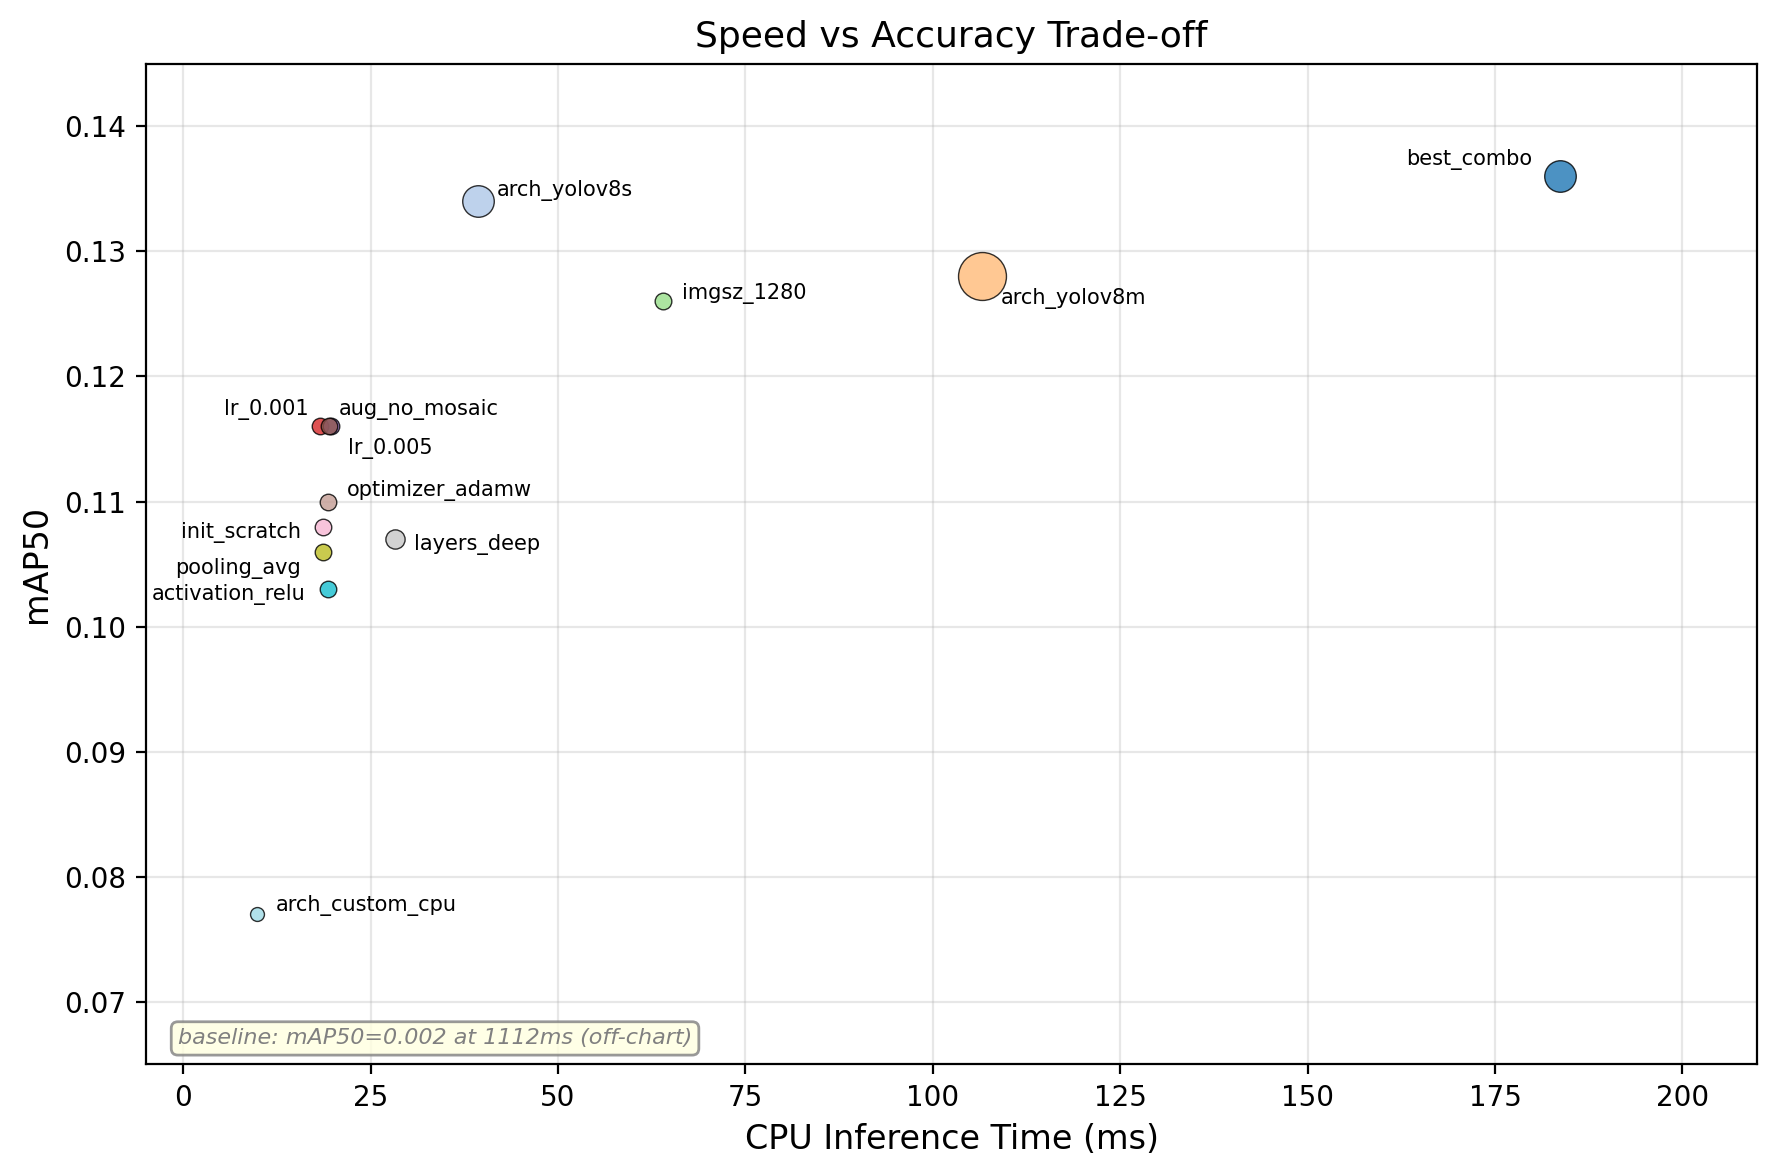
\includegraphics[width=0.48\textwidth]{figures/speed_vs_accuracy.png}
\hfill
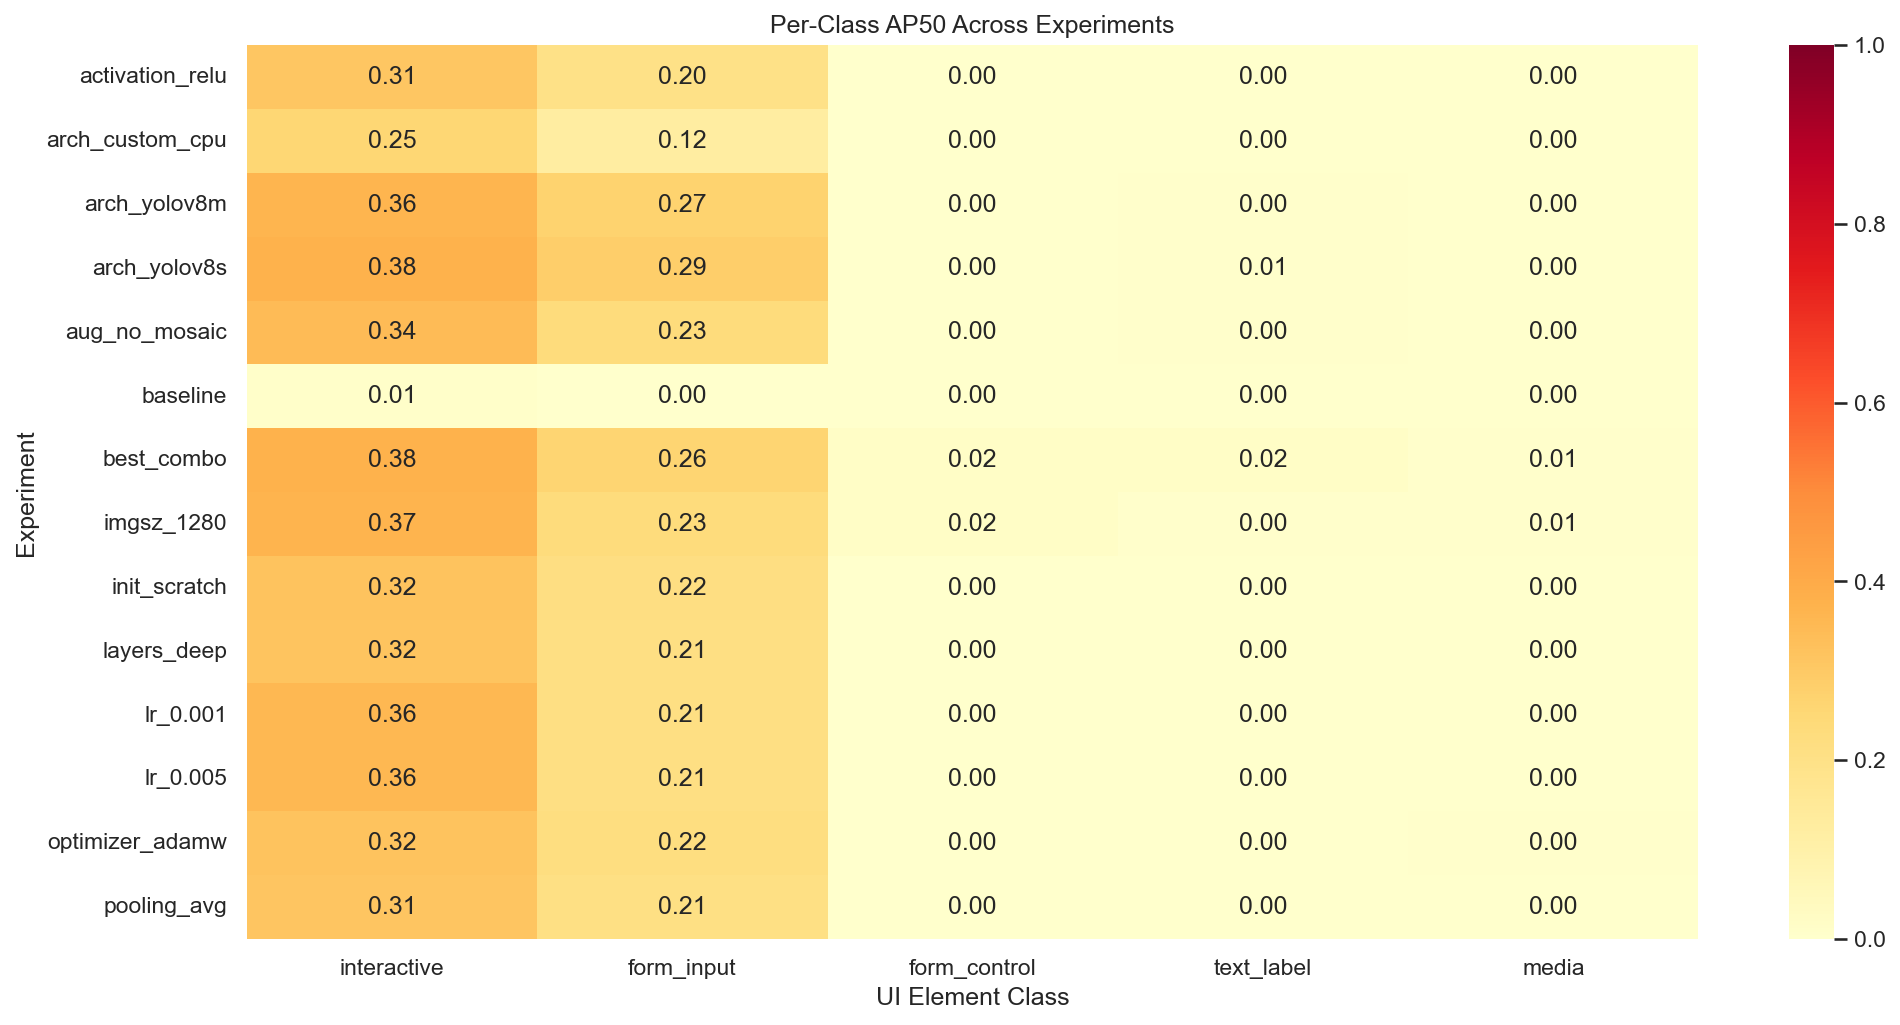
\includegraphics[width=0.48\textwidth]{figures/per_class_ap.png}
\caption{\textbf{Left:} Speed--accuracy trade-off across the 14 CNN ablation experiments. \textbf{Right:} Per-class AP50 heatmap showing that only \texttt{interactive} and \texttt{form\_input} are consistently detected in the 5-class setting, motivating the 1-class consolidation.}
\label{fig:yolo_figures}
\end{figure*}

\subsection{Discussion}

\textbf{OmniParser replication.} Our 1-class results independently confirm that YOLOv8 with single-class detection works for UI elements, matching OmniParser's design choice. The difference is we provide a systematic ablation showing \textit{why} it works---multi-class detection fails due to class imbalance, not model limitations.

\textbf{Validated defaults.} SiLU $>$ ReLU (+0.005 mAP50) and max pooling $>$ average pooling (+0.002) are small but consistent. YOLOv8's default component choices are well-tuned.

% ============================================================
\section{Conclusion}

We trained YOLOv8 for UI element detection in web screenshots, conducting 14 ablation experiments across all five standard CNN hyperparameter categories---architectures, layers, optimizers, pooling, and activations. Architecture choice had the largest effect among hyperparameters, but the real breakthrough came from data refinement: consolidating 16 noisy classes into 1 clean class with deduplication and diverse sampling improved mAP50 from 0.136 to 0.323 (2.4$\times$), confirming OmniParser's single-class approach on independent data.

The main takeaway for training CNNs on new tasks: invest in data quality before hyperparameter tuning. Our 14-experiment ablation changed mAP50 by at most 0.03 across all axes, while fixing the data pipeline produced a 0.19 gain.

% ============================================================
\section{Practical Extension: Text Classifier}
\label{sec:classifier}

Beyond the core CNN work, we explored a practical application: detecting prompt injection attacks in the text content of UI elements. YOLO finds the elements; OCR extracts their text; a classifier flags malicious content.

We trained a DeBERTa-v3-xsmall~\cite{deberta} text classifier (22M parameters) using focal loss~\cite{focalloss} ($\gamma=2.0$, $\alpha=[0.7,0.3]$)---a variant of cross-entropy that down-weights easy examples so the model focuses on hard cases, which helps when most text is clearly benign. We trained on 23K balanced examples from six public sources. We ran 17 additional ablation experiments across architecture, loss function, class weighting, sequence length, and data composition. Table~\ref{tab:classifier_benchmarks} compares against two published baselines on independent benchmarks with zero training data overlap.

\begin{table}[h]
\caption{Text classifier on independent benchmarks. Our 22M-parameter model outperforms larger baselines on most benchmarks.}
\label{tab:classifier_benchmarks}
\centering
\small
\begin{tabular}{llrrr}
\toprule
Benchmark & Metric & Ours & ProtectAI & Meta \\
 & & (22M) & (200M) & (86M) \\
\midrule
NotInject EN (253) & Acc & \textbf{89.3} & 62.5 & 0.0 \\
 & FPR & \textbf{10.7} & 37.5 & 100.0 \\
\midrule
Wildguard (971) & Acc & \textbf{97.8} & 75.2 & 6.7 \\
 & FPR & \textbf{2.2} & 24.8 & 93.3 \\
\midrule
Gandalf (112) & Recall & 92.0 & \textbf{100.0} & \textbf{100.0} \\
\midrule
InjecGuard (144) & Acc & \textbf{71.5} & 65.3 & 43.8 \\
\bottomrule
\end{tabular}
\end{table}

For deployment, we exported to ONNX with INT8 quantization, reducing latency from 16.1ms to 3.8ms (4.2$\times$ speedup) and model size from 271~MB to 83~MB.

Development of the report and scripts was assisted by Claude Code.

% ============================================================
\bibliography{main}
\bibliographystyle{icml2023}

\end{document}
